\documentclass[9pt, table]{beamer}

\usepackage[slovene]{babel}
\usepackage{ifthen} 
\usepackage[utf8]{inputenc}
\usepackage[T1]{fontenc}
\usepackage{lmodern}


\usepackage{mathptmx}
\usepackage{helvet}
\usepackage{courier}


\usetheme{Warsaw}
\useoutertheme{infolines}
\usecolortheme{seahorse}
\setbeamercovered{transparent}


\newtheorem{trd}{Trditev}
\newtheorem{izr}{Izrek}
\newtheorem{lema}{Lema}
\renewenvironment{proof}{\textit{Dokaz:}}{$\Box$}

\theoremstyle{remark}
\newtheorem*{op}{Opomba}
\newtheorem*{posl}{Posledica}

\theoremstyle{definition}
\newtheorem{defi}{Definicija}

\definecolor{softyellow}{rgb}{0.98,0.98,0.75}
\setbeamercolor{lowercol}{fg=black,bg=softyellow}

\title[Grupa kit] {Grupa kit in njene upodobitve}
\subtitle{Predstavitev pri diplomskem seminarju}
\author{Živa Urbančič}
\institute[FMF] {Fakulteta za matematiko in fiziko}
\date{14. november 2016}

\begin{document}

\begin{frame}
  \titlepage
\end{frame}

% -------------------------------------------------------------------
\section{Zgodovina}
\begin{frame}
\frametitle{Zgodovina}
\begin{columns}
\begin{column}[T]{5cm}
\begin{figure}
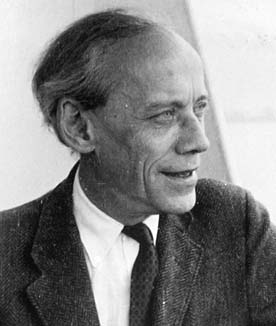
\includegraphics[height = 4.5cm]{Emil_Artin}
\caption{Emil Artin, 1898 - 1962}
\end{figure}
\end{column}
\begin{column}[T]{5cm}
\begin{itemize}
\item Povezanost s teorijo vozlov.
\item E. Artin: \emph{Theorie der Zopfe}, 1925.
\item E. Artin: \emph{Theory of braids}, 1946.
\end{itemize}
\end{column}
\end{columns}
\end{frame}

% -------------------------------------------------------------------
\section{Grupa kit}
\begin{frame}
\frametitle{Geometrijska definicija}
Na premicah $\{y = z = 0\}$ ter $\{y = 0,\ z = 1\}$ v $\mathbb{R}^3$ izberemo $m$ točk z abscisami $x=1,\ 2,\ \ldots,\ m$.
\vspace{0.2cm}
\pause
\begin{defi}
\emph{Kita z m prameni} je množica $m$ disjunktnih gladkih poti - \emph{pramenov}, ki povezujejo točke s prve izbrane premice s tistimi z druge (v poljubnem vrstnem redu).  Projekcija vsakega pramena na os $z$ mora biti difeomorfizem.
\end{defi}
\vspace{0.5cm}
\begin{figure}
\only<2>{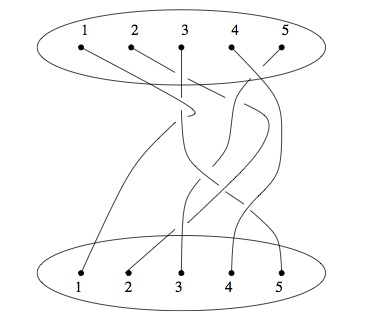
\includegraphics[height = 3cm]{Primer_kite_1}}
\caption{Primer kite s 5 prameni.}
\end{figure}
\end{frame}

%--------------------------------------------------------------------
\begin{frame}
\frametitle{Ekvivalenca kit}
\begin{defi}
Kiti $B_0$ in $B_1$ sta \emph{ekvivalentni}, če sta \emph{izotopni}.
\end{defi}
\pause
\begin{op}
Eno vložitev kite lahko zvezno deformiramo v drugo.
\end{op}
\end{frame}

%--------------------------------------------------------------------
\begin{frame}
\frametitle{Ali imamo grupo?}
\pause
\begin{trd}
Množica ekvivalenčnih razredov kit z m prameni za operacijo stikanja generira grupo.
\end{trd}
\begin{columns}
\begin{column}{5cm}
\only<2,3>{
\begin{figure}
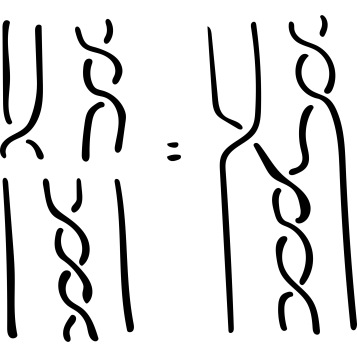
\includegraphics[height=4cm]{Stikanje_1}
\caption{Stikanje.}
\end{figure}}
\end{column}
\begin{column}{5cm}
\only<3>{
\begin{figure}
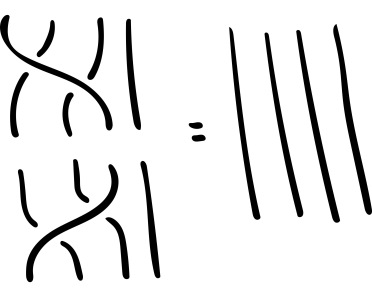
\includegraphics[height=4cm]{Inverz_1}
\caption{Inverzni element in enota.}
\end{figure}}
\end{column}
\end{columns}
\end{frame}
%--------------------------------------------------------------------

\begin{frame}
\frametitle{Algebraična definicija}
\begin{defi}
\emph{Grupa kit z m prameni} je podana z $(m-1)$ generatorji $\sigma_1,\ \ldots,\ \sigma_{m-1}$ in naslednjimi relacijami: $$\sigma_i \sigma_j = \sigma_j \sigma_i$$ za $|i - j| \geq 2$ in $$\sigma_i \sigma_{i+1} \sigma_i= \sigma_{i+1} \sigma_i \sigma_{i+1}$$ za vse $i = 1,\ \ldots,\ m-2$.
\end{defi}
\end{frame}

% -------------------------------------------------------------------
\begin{frame}
\frametitle{Uporaba}
\begin{itemize}
\item{Mehanika fluidov.}
\item{Statistična mehanika.}
\item{Kriptografija.}
\item{Reševanje polinomskih enačb.}
\end{itemize}
\end{frame}

\begin{frame}
\begin{figure}[c!]
Naslednjič ...
\end{figure}
\end{frame}

\section{Literatura}
\begin{frame}
\frametitle{Literatura}
\begin{itemize}
\item G. Burde, H. Zieschang. {\em Knots}, 2nd ed. Walter de Gruyter, Berlin, 2003.
\item V. O. Manturov. {\em Knot Theory}, 1st ed. CRC Press, 2004. Dostopno na \url{http://varf.ru/rudn/manturov/book.pdf}.
\item{\emph{Braid theory}, v: Wkipedia: The Free Encyclopedia, [ogled 11. 11. 2016], dostopno na \url{https://en.wikipedia.org/wiki/Braid_theory}}
\end{itemize}
\end{frame}


\end{document}